\documentclass[10pt,a4paper,french,titlepage]{article}
\author{par Gabriel Caux et Léo Peyronnet : Binome numéro 3}
\title{La réussite des alliances}
\date{Février-Avril 2022}
\usepackage[utf8]{inputenc}
\usepackage[T1]{fontenc}
\usepackage{babel}
\usepackage{amsfonts}
\usepackage{amsthm}
\usepackage{mathtools}
\usepackage{amssymb}
\usepackage{listings}
\usepackage[pdftex]{hyperref}
\usepackage{amssymb}
\usepackage{tabto}
\usepackage{pst-node}
\usepackage{listings}
\lstset{
  aboveskip=3mm,
  belowskip=-2mm,
  basicstyle=\footnotesize,
  breakatwhitespace=false,
  breaklines=true,
  captionpos=b,
  commentstyle=\color{red},
  deletekeywords={...},
  escapeinside={\%*}{*)},
  extendedchars=true,
  framexleftmargin=16pt,
  framextopmargin=3pt,
  framexbottommargin=6pt,
  frame=tb,
  keepspaces=true,
  keywordstyle=\color{blue},
  language=C,
  literate=
  {²}{{\textsuperscript{2}}}1
  {⁴}{{\textsuperscript{4}}}1
  {⁶}{{\textsuperscript{6}}}1
  {⁸}{{\textsuperscript{8}}}1
  {€}{{\euro{}}}1
  {é}{{\'e}}1
  {è}{{\`{e}}}1
  {ê}{{\^{e}}}1
  {ë}{{\¨{e}}}1
  {É}{{\'{E}}}1
  {Ê}{{\^{E}}}1
  {û}{{\^{u}}}1
  {ù}{{\`{u}}}1
  {â}{{\^{a}}}1
  {à}{{\`{a}}}1
  {á}{{\'{a}}}1
  {ã}{{\~{a}}}1
  {Á}{{\'{A}}}1
  {Â}{{\^{A}}}1
  {Ã}{{\~{A}}}1
  {ç}{{\c{c}}}1
  {Ç}{{\c{C}}}1
  {õ}{{\~{o}}}1
  {ó}{{\'{o}}}1
  {ô}{{\^{o}}}1
  {Õ}{{\~{O}}}1
  {Ó}{{\'{O}}}1
  {Ô}{{\^{O}}}1
  {î}{{\^{i}}}1
  {Î}{{\^{I}}}1
  {í}{{\'{i}}}1
  {Í}{{\~{Í}}}1,
  morekeywords={*,...},
  numbers=left,
  numbersep=10pt,
  numberstyle=\tiny\color{black},
  rulecolor=\color{black},
  showspaces=false,
  showstringspaces=false,
  showtabs=false,
  stepnumber=1,
  stringstyle=\color{gray},
  tabsize=4,
  title=\lstname,
}


\begin{document}
\maketitle
\tableofcontents
\section{La réussite des alliances: structuration du jeu}
\subsection{Rappel des règles du jeu}
Quelque rappel des règles:\\
Prenez un paquet de cartes (32 ou 52) mélangez le pour créer une pioche, ensuite tirez les cartes une par une en les posant de gauche a droite faces visibles. Une fois que trois cartes ont été posées vous pouvez commencer à jouer. On procédera ainsi, on suppose que la carte la plus a gauche est la numéro une la carte à sa droite la numéro deux celle a sa droite numéro trois et ainsi de suite. Si la carte numéro trois a une similarité (même couleur ou même valeur) avec la carte numéro une il y a alors alliance de cartes, vous pouvez alors faire un saut dans ce cas la la carte qui est située entre nos deux cartes passe sur le tas de celle qui l'a précède. Si aucun saut n'est possible il faudra continuer à piocher les cartes jusqu'à ce qu'un ou plusieurs saut soit possible le jeu s'arrête lorsqu'il n'est plus possible de piocher une carte et qu'il n'est pas possible de faire de saut non plus. On compte alors le nombre de tas restant et selon le nombre de tas requis pour gagner vous savez si oui ou non vous avez réussi.\\\\

\subsection{Création des fonctions (partie guidée)}
Pour représenter informatiquement le jeu de la réussite des alliances, nous avions à notre disposition une partie guidée intégrée au sujet.
Ce "cahier des charges" détaillé nous a fourni un certain confort quant à l'architecture du programme en lui même. En effet, comme les entrées, 
sorties et effets de bords de nos fonctions nous étaient déjà indiqué, nous n'avions pas à réfléchir à comment nos fonctions allaient interagir entre elles. Les appels à des fonctions antérieures, s'il en avait, nous étaient eux aussi indiqués ou tout du moins suggérés. Cette souplesse de travail nous
a permis de nous concentrer sur l'algorithmique de nos fonctions et comment optimiser ces dernières.\\

Néanmoins, le sujet nous permettait également de prendre certaines libertés. Par exemple, il nous était suggéré de réaliser des fonctions
auxiliaires pour programmer la fonction "$une\_etape\_reussite$". C'est ce que nous avons fait avec la fonction "$piocher$" qui compartimente l'action de 
piocher une carte. Elle prends en argument deux listes, une qui représente la liste des tas de la réussite, l'autre qui représente la pioche. Elle a 
pour effet de bord de déplacer la première carte de la pioche (c'est à dire d'indice 0) au dernier emplacement de la liste des tas. Pour cela, nous 
avons utilisé la fonction "$pop$" qui a elle même pour effet de bord de supprimer un élément d'une liste à un index précis et qui retourne cet élément.
Nous avons donc redirigé la sortie de la fonction "$pop$" comme ceci:\\
\begin{lstlisting}
	def piocher(liste_tas,pioche):
    		liste_tas+=[pioche.pop(0)]

\end{lstlisting}
\caption{fonction : ligne 118\\} 

Nous n'avons cependant pas jugé nécéssaire de faire d'autres compartimentations pour fluidifier cette fonction.\\

La fonction "$reussite\_mode\_manuel$" nous a permis à nouveau de pouvoir prendre des libertés cette fois-ci quant à l'affichage des éléments et
plus globalement l'interface utilisateur. Pour rappel, cette fonction a pour but de laisser l'utilisateur jouer une partie. Ceci nécessite une interface
pour que l'utilisateur puisse choisir ce qu'il veut faire. Ainsi, afin de présenter au mieux ses options de jeu à l'utilisateur, nous avons réaliser un
menu contenant un choix pour piocher, un choix pour réaliser un saut et un choix pour mettre fin à la partie. En plus de ce menu, nous avons décider de
réaliser un affichage de la réussite plus poussé permettant de relier chaque carte à un nombre et ainsi faciliter la sélection de la carte à faire
sauter. Pour cela, nous avons réaliser la fonction "$afficher\_reussite\_num$". Elle prends pour argument la liste de cartes à afficher, ne revoie rien et a pour effet de bord l'affichage détaillé de la réussite. Cette fonction consiste en 3 boucles affichant respectivement les cartes de la réussite, les
accents circonflexes permettant de souligner les cartes, et les nombres désignant les cartes. A noter que bien que semblant être des index, ces nombres
n'en sont pas tout à fait car: soit une liste $li$, $u$ l'index d'un élément de cette liste et $v$ un des nombres utilisés dans la fonction , alors:
\begin{align*}
	&u \in [0;(len(li)-1)] \iff [0;len(li)[\\
	&v \in [1;len(li)]
\end{align*}

Lors de la création de cette fonction, nous avons constater des bugs survenant lors de l'affichage de grandes listes de cartes comme par exemple une pioche entière d'un jeu de 52 cartes. A raison de 4 caractères imprimés par carte (les 3 caractères de la carte $+$ l'espace de fin du print), l'affichage entier d'un jeu de 52 cartes correspond à l'impression de $4\times52=208$ caractères. Cela peut être un problème si l'utilisateur possède un petit écran et par conséquent un petit terminal. Les trois lignes de 208 caractères peuvent "déborder" chacune leur tour, provoquant des bugs similaires à  celui-ci:\\\\
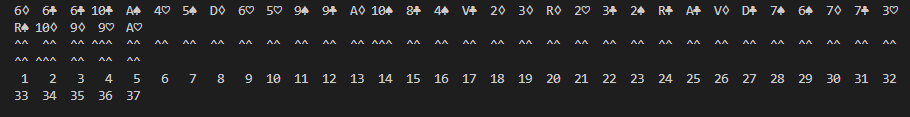
\includegraphics[scale=0.5]{img/bug_afficher_reussite_num.PNG}

Nous avons résolu ce problème en imbriquant les trois boucles d'affichage dans une plus grande boucle, et en changeant la condition de la première boucle. Maintenant, la première boucle conditionne les deux suivantes puisqu'elles sont des boucles "$for$" tournant sur une liste ($li\_dix$) ayant un nombre  d'éléments équivalent au nombre de passage dans la première boucle. Cette boucle s'arrête soit lorsqu'il n'y a plus de cartes dans la liste, soit si l'affichage dépasse la taille du terminal. Le compteur "$y$" est incrémenté à chaque passage dans la boucle, c'est à dire à chaque impression de carte. Il permet donc de savoir où nous en sommes dans la lecture/impression de la réussite et par conséquent, poser une condition de sortie de boucle lorsque qu'on arrive au bout de la liste de cartes. Le compteur "$i$" qui est incrémenté lui aussi à chaque impression mais réinitialisé à chaque passage dans la grande  boucle (ce qui reviens à une ré-initialisation à la sortie de la "petite" boucle). Donc, multiplié par 4, il permet de compter le nombre de caractères imprimés à chaque passage de grande boucle. Il faut maintenant connaître la largeur du terminal pour pouvoir la comparer à "$i$". Pour obtenir la taille du terminal, nous avons utilisé le module intégré à python: "$shutil$". Avec la fonction "$get\_terminal\_size$", on peut obtenir le nombre de caractères que peut  contenir le terminal en longueur. Ainsi, nous pouvons construire la deuxième condition de sortie de boucle en spécifiant que la boucle est valide tant que $i \times 4$ est inférieur ou égal à la largeur du terminal. Après modifications, la fonction est donc comme suit :
\begin{lstlisting}
def afficher_reussite_num(liCartes):
    columns, rows = shutil.get_terminal_size()
    i=0
    y=0
    li_dix=[]
    cpt=1
    while y<len(liCartes):
        i=1
        li_dix=[]
        while i*4<=columns and y<len(liCartes): 
            carte=liCartes[y]
            print(carte_to_chaine(carte),end=" ")
            if carte["valeur"]==10:
                li_dix+=[True]
            else:
                li_dix+=[False]
            y+=1
            i+=1
        print()
        for dix in li_dix:
            if dix:
                print("^"*3,sep="",end=" ")
            else:
                print(" ","^"*2,sep="",end=" ")
        print()
        for dix in li_dix:
            if cpt<10:
                print(" "*2,cpt,sep="",end=" ")
            else:
                print(" ",cpt,sep="",end=" ")
            cpt+=1
        print("\n")
\end{lstlisting}
\caption{fonction: ligne 24}



\section{Les Extensions: ajouts de fonctionnalités.}
\subsection{Vérification de la pioche}
Parmi les idées d'extensions que propose le sujet, nous avons choisi la fonction permettant de vérifier que la pioche de cartes ne soit pas truquée. Nommée "$vérifier\_pioche$", elle prends en arguments la liste que l'on souhaite vérifier ainsi que le nombre de cartes qu'elle contient - ou tout du moins qu'elle est censée contenir ! Elle n'a pas d'effets de bord et renvoie un booléen pour statuer de la conformité de la pioche: True si la pioche est conforme et False si la pioche est truquée. Notre algorithme se base sur la comparaison de la liste passée en argument avec une liste conforme. Une pioche peut être truquée de différentes manières:
\begin{itemize}
\item on peut ajouter les cartes que l'on souhaite directement dans la liste, auquel cas la taille de la liste doit être trop grande.\\
\item on peut sinon placer les cartes que l'on souhaite à l'index d'une autre carte. On remplace donc une carte par une autre, ce qui reviens à réécrire les cartes pour qu'elles nous arrangent. Il faudra donc veiller à ce qu'il n'y est pas de double. Pour cela, et comme nous savons que la taille de la liste sera contrôlé ensuite, il nous suffit juste de veiller à ce que toutes les cartes présentes dans une pioche conventionnelle le soit aussi dans la pioche que l'on contrôle. Ainsi, s'il y a des doubles, cette dernière sera forcement d'une taille non conforme.\\
\end{itemize}

Nous avons donc fait appel à notre fonction "$init\_pioche\_alea$" crée lors de la partie guidée qui permet de générer une pioche de 32 ou 52 cartes mélangées aléatoirement\label{piochealea}. Cette pioche nous sert donc de comparaison. Nous passons tout d'abord en revue la pioche suspecte en veillant à ce que chaque carte de la pioche conforme soit dans la pioche suspecte. Si ce n'est pas le cas, la fonction renvoie False. La fonction procède ensuite à une vérification de la longueur de la pioche suspecte. Pareil, si la pioche a plus de cartes qu'elle ne devrait en avoir, la fonction renvoie False. Si la pioche possède toutes les cartes de la pioche conforme tout en ayant le bon nombre de cartes, alors la fonction renvoie True.\\

\subsection{Statistiques}
Nous avons aussi choisi deux fonctions liées aux statistiques : \\La première étant nommée "$res\_multi\_simulation$" qui va comme son nom l'indique nous servir à faire de multiples simulations de parties en même temps. Elle prend en argument le nombre de simulation que nous voulons faire ainsi que le nombre de carte que notre jeu contient. Voilà comment cette fonction procède, elle crée d'abord une boucle qui va faire appel à deux fonctions de la partie guidée, "$init\_pioche\_alea$" qui comme décrite précédemment génère une pioche de 32 ou 52 cartes mélangées aléatoirement ainsi que "$reussite\_mode\_auto$" qui permet de jouer une partie de réussite des alliances automatiquement. Ces deux fonctions nous permettent de faire des simulations différentes à chaque boucle. Après avoir fait chaque simulation de partie elle rajoute le résultat dans une liste qui est finalement renvoyée à la fin de la fonction. Cette liste qui est renvoyée correspond donc aux nombres de tas restants pour chaque simulation.
\\
La seconde fonction se nomme "$statistiques\_nb\_tas$" elle va nous servir à connaitre certaines statistiques. Elle prend en argument le nombre de simulation que nous souhaitons faire ainsi que le nombre de carte contenu dans le jeu (32 ou 52). \\ 
Cette fonction a pour but de faire un nombre défini de simulation puis de trouver ou calculer la moyenne, le maximum ainsi que le minimum de tas obtenus. Pour faire cela elle va d'abord faire appel a la fonction "$res\_multi\_simulation$" vu précédemment qui va servir à donner une liste depuis laquelle nous allons pouvoir calculer les statistiques dont nous avons besoins pour cela nous allons créer une boucle qui va nous servir à trois choses:
\begin{itemize}
\item premièrement grâce à cette boucle nous allons pouvoir additionner toutes les valeurs d'une liste dans une seul variable.
\item nous allons aussi pouvoir trouver le maximum et le minimum en comparant les valeurs entre elles.
\end{itemize}
Une fois sorti de cette boucle nous pouvons alors diviser notre variable moyenne par la longueur de la liste pour trouver la moyenne. Cette fonction nous affiche donc la moyenne, le maximum et le minimum de tas pour un nombre prédéfinis de simulations.

\subsection{Probabilités}
\section{Le debug$\_$mode}
\subsection{Naissance de la nécessité de pouvoir tester les fonctions}
\subsection{Structure du programme}
\subsection{Limites et Erreurs}
\section{Interface utilisateur: proposer un produit fini.}
\section{Annexes}



Le liens de notre gitlab est :\url{https://gitlab.isima.fr/lepeyronne/la-reussite-des-alliances}
\end{document}
